% Preamble ==================================================================
\documentclass[11pt]{article}
\usepackage{geometry}
\geometry{verbose,tmargin=2.5cm,bottom= 1.5cm,lmargin=2.5cm,rmargin=2.5cm}
\usepackage{float}
\usepackage{graphicx}
\usepackage{amsmath}
\usepackage{amssymb}
\usepackage{enumitem}
\usepackage{mathtools}

\usepackage{amsthm} % theorem
\usepackage{listings} % code snippets
\usepackage{fancyvrb} %verbatim
\lstset{frame=l,
  language=Python,
  basicstyle={\small\ttfamily},
  numbers=none,
  numberstyle=\tiny\color{black},
  keywordstyle=\color{black},
  commentstyle=\color{blue},
  stringstyle=\color{mauve},
}

\numberwithin{equation}{section}

\usepackage{titlesec,dsfont}

%Format section heading style
\usepackage{sectsty}
\sectionfont{\sffamily\bfseries\large}
\subsectionfont{\sffamily\normalsize\slshape}
\subsubsectionfont{\sffamily\small\itshape}
\paragraphfont{\sffamily\small\textbf}


%Put period after section number
\makeatletter
\def\@seccntformat#1{\csname the#1\endcsname.\quad}
\makeatother

%Bibliography
\usepackage[round]{natbib}
\bibliographystyle{genetics}

%Format captions
\usepackage[ labelsep=period, justification=raggedright, margin=10pt,font={small},labelfont={small,normal,bf,sf}]{caption}

\setlength{\parskip}{0ex} %No space between paragraphs.

\renewcommand{\familydefault}{\sfdefault}

\newcommand\indep{\protect\mathpalette{\protect\independenT}{\perp}}
\newcommand{\nindep}{\not\!\perp\!\!\!\perp}
\def\independenT#1#2{\mathrel{\rlap{$#1#2$}\mkern2mu{#1#2}}}

%PUT ME LAST--------------------------------------------------
\usepackage[colorlinks=true
,urlcolor=blue
,anchorcolor=blue
,citecolor=blue
,filecolor=blue
,linkcolor=black
,menucolor=blue
,linktocpage=true
,pdfproducer=medialab
,pdfa=true
]{hyperref}

\makeatother %Put this last of all


\newcommand{\defeq}{\coloneqq}
\newcommand{\overbar}[1]{\mkern 1.5mu\overline{\mkern-1.5mu#1\mkern-1.5mu}\mkern 1.5mu}

% Make theorems bold
\makeatletter
\def\th@plain{%
  \thm@notefont{}% same as heading font
  \itshape % body font
}
\def\th@definition{%
  \thm@notefont{}% same as heading font
  \normalfont % body font
}
\makeatother

\newtheorem{thm}{Theorem}[section]
\newtheorem{defn}{Definition}[section]
\newtheorem{cor}{Corollary}[section]
\newtheorem{prop}{Property}[section]
\newtheorem{rle}{Rule}[section]
\newtheorem{lma}{Lemma}[section]

%Preamble end--------------------------------------------------


\begin{document}

\begin{flushleft}
\textbf{\Large Sequence models}
\end{flushleft}

\begin{flushleft}
Author: Juvid Aryaman

Last compiled: \today
\end{flushleft}

\noindent This document contains my personal notes on sequence models.


\section{Embeddings}
Embeddings are tensors. You interact with that tensor by indexing into it. It is often used to store encodings of collections of words. For example:
\begin{lstlisting}
>>> nn.Embedding(vocab_sz, n_hidden)
\end{lstlisting}	
creates a set of \verb#vocab_sz# tensors, each of size \verb#n_hidden#. 

A common thing to do is to something like:
\begin{lstlisting}
>>> embedding = nn.Embedding(10, 3)
>>> input = torch.LongTensor([[1,2,4,5],[4,3,2,9]])
>>> embedding(input)

tensor([[[-0.0251, -1.6902,  0.7172],
         [-0.6431,  0.0748,  0.6969],
         [ 1.4970,  1.3448, -0.9685],
         [-0.3677, -2.7265, -0.1685]],

        [[ 1.4970,  1.3448, -0.9685],
         [ 0.4362, -0.4004,  0.9400],
         [-0.6431,  0.0748,  0.6969],
         [ 0.9124, -2.3616,  1.1151]]])
\end{lstlisting}
so you can see that the input is \verb#[sentence1, sentence2]#, where sentence 1 consists of words \verb#[1,2,4,5]#. As an output, we get the corresponding 3-vectors for each word. So the output is: 
\begin{lstlisting}
[[[embedding_word_1,   # length 3 vector
   embedding_word_2, 
   embedding_word_4, 
   embedding_word_5],
  
  [embedding_word_4, 
   embedding_word_3, 
   embedding_word_2, 
   embedding_word_9]
]]
\end{lstlisting}

\section{Linear layer}
Applies a linear transformation to the incoming data: $y = xA^T + b$
\begin{lstlisting}
>>> m = nn.Linear(20, 30)
>>> input = torch.randn(128, 20)
>>> output = m(input)
>>> print(output.size())
torch.Size([128, 30])
\end{lstlisting}


\section{Recurrent neural network}
Torch, by default, applies a multi-layer Elman RNN. This is defined as applying the following function to each element of the input sequence
\begin{align}
h_t  &= \sigma_h(W_h x_t + U_h h_{t-1} + b_h)\\
y_t  &= \sigma_y(W_y h_t + b_y)
\end{align}
where $x_t$ is an input vector, $h_t$ is a hidden layer vector, $y_t$ is an output vector, $W, U, b$ are parameter matrices and vector, $\sigma_h, \sigma_y$ are activation functions. Note that we don't actually retain the hidden state between lines -- we throw it away after every complete training example (a line). We will typically initialize the hidden state to be $h_{t=0}=0$. Within a particular training instance, on a particular line, we may have different maximum values of $t=T$. 

For example, in word classification, where we construct a character-level RNN, in each training loop we will
\begin{enumerate}[noitemsep]
\item Get an input and target tensor
\item Create a zeroed initial hidden state
\item Read each letter in and:
\begin{itemize}[noitemsep]
\item Keep hidden state for next letter
\item Feed the previous hidden state $h_{t-1}$ in with the current input $x_t$
\end{itemize}
\item Compare output at the end of the RNN loop to the target
\item Back-propagate
\end{enumerate}
Then return the output and loss.

\begin{figure}
\begin{center}
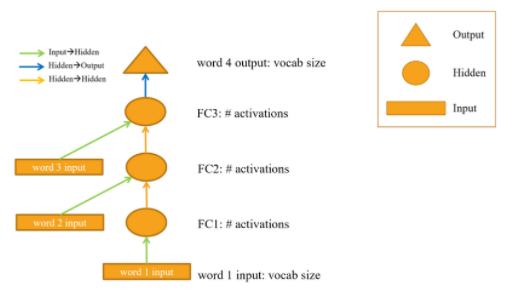
\includegraphics[width=0.8\columnwidth]{../figures/rnn.png}  
\end{center}
\caption{Graphical representation of RNN
}
\label{fig:rnn}
\end{figure}

\subsection{Gated recurrent unit}
A GRU is a type of RNN. They are similar to LSTMs but have fewer parameters and can be easier to train. The key innovation is that they allow the network to control the amount of information which flows between consecutive time steps, and allows the network to forget. 

For each element in the input sequence, each layer computes the following function:
\begin{align}
z_t &= \sigma(W_{iz}x_t + b_{iz} + W_{hz} h_{(t-1)} + b_{hz}) \label{eq:gru_update_gate_zt} \\
r_t &= \sigma(W_{ir}x_t + b_{ir} + W_{hr}h_{(t-1)} + b_{hr}) \label{eq:gru_reset_gate_rt} \\
n_t &= \tanh(W_{in} x_t + b_{in} + r_t \odot (W_{hn} h_{(t-1)} + b_{hn}) ) \label{eq:gru_candidate_hidden_state_nt} \\
h_t &= (1-z_t) \odot n_t + z_t \odot h_{(t-1)} \label{eq:update_ht}
\end{align}
where $x_t$ is the input at time $t$, $h_t$ is the hidden state at time $t$. $r_t$, $z_t$, and $n_t$ are the reset, update, and new gates respectively. $\sigma$ is the sigmoid function, and $\odot$ is the Hadamard product.

\begin{figure}
\begin{center}
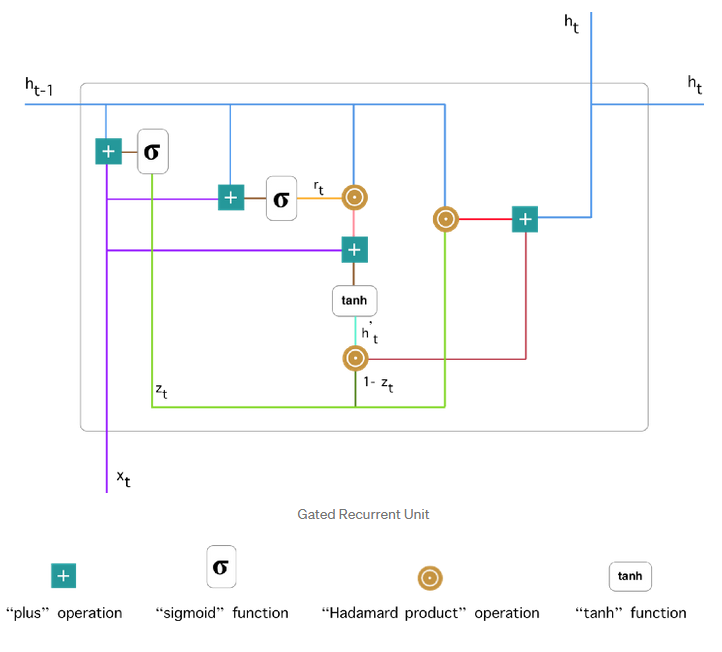
\includegraphics[width=0.8\columnwidth]{../figures/gru.png}  
\end{center}
\caption{Graphical representation of GRU. I don't actually find these super-helpful.
}
\label{fig:rnn}
\end{figure}

\begin{enumerate}[noitemsep]
\item Eq.\eqref{eq:gru_update_gate_zt} is called the \textbf{update gate}. The update gate combines the input with the previous hidden state. It determines how much of the previous step's hidden state $h_{t-1}$ is passed onto the new hidden state $h_{t}$ in Eq.\eqref{eq:update_ht}.
\item Eq.\eqref{eq:gru_reset_gate_rt} is called the \textbf{reset gate}. The formula is the same as Eq.\eqref{eq:gru_update_gate_zt}. It will be used to decide how much of the past information to \textbf{forget} in Eq.\eqref{eq:gru_candidate_hidden_state_nt}.
\item Eq.\eqref{eq:gru_candidate_hidden_state_nt} is a \textbf{candidate} hidden state. It combines the current input with some weighting of the previous hidden state. The reset gate $r_t$ has an element-wise product with $h_{t-1}$, allowing the network to forget $h_{t-1}$ as $r_t \rightarrow 0$. 
\item Eq.\eqref{eq:update_ht} mixes the previous hidden state $h_{t-1}$ with the candidate hidden state $n_t$ through a convex combination weighted by $z_t$.
\end{enumerate}

\section{Attention}
\subsection{Bahdanau attention}
\cite{bahdanau14} were the first to describe an attention model in the context of an encoder-decoder recurrent model. The model is broadly as follows. An encoder reads an input sequence of vectors $x=(x_1,...,x_{T_x})$, where each element corresponds to e.g. a word in a sentence and the vector is an embedding vector with some fixed embedding dimension. They use an RNN to generate a hidden state $h_t \in \mathbb{R}^n$ for each time $t$
\begin{equation}
h_t = f(x_t, h_{t-1})
\end{equation}
and a context vector which, in general, is written as
$c = q(\{h_1,...,h_{T_x}\})$
where both $f$ and $q$ are some non-linear functions. We concatenate the forwards and backwards hidden states of a bidirectional GRU in \verb#seq.enc_dec_attn# to form $c$, see Fig.~\ref{fig:bah-attn}.

\begin{figure}
\begin{center}
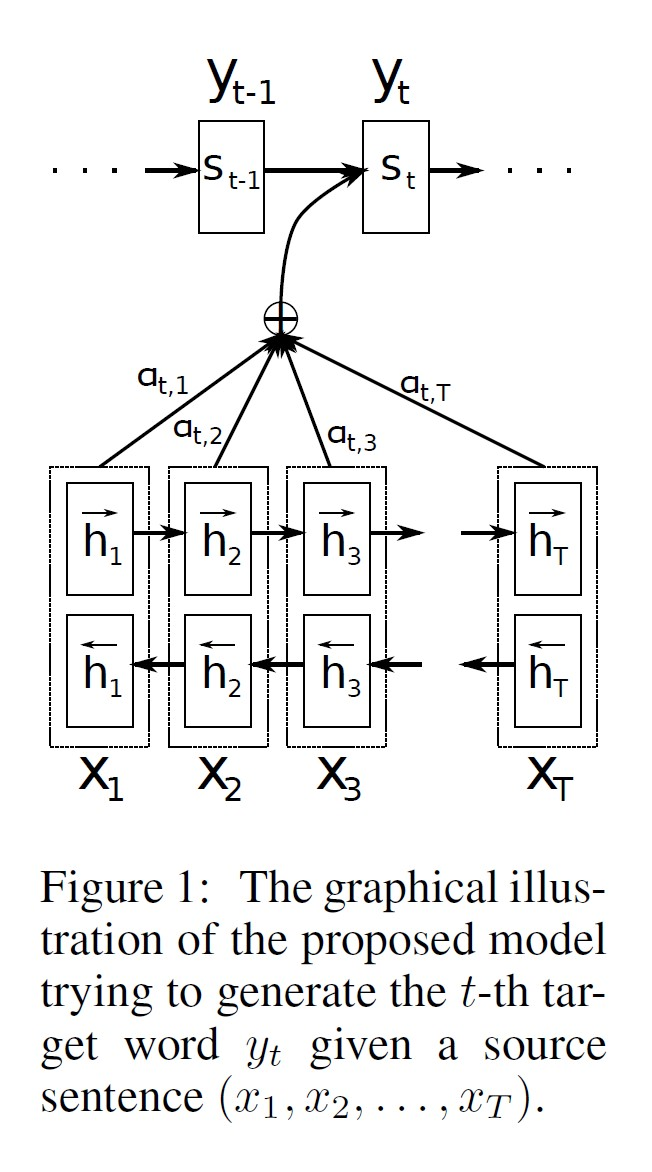
\includegraphics[width=0.4\columnwidth]{../figures/enc-dec-attn.jpg}  
\end{center}
\caption{Bahdanau attention \citep{bahdanau14}, depicting Eq.\eqref{eq:bah-dec-hidden} and Eq.\eqref{eq:bah-attn-mech} graphically.}
\label{fig:bah-attn}
\end{figure}

For the decoder, we have a sequence of target vectors $y=(y_1,...,y_{T_y})$ and an RNN hidden state $s_i$ where
\begin{equation}
s_i = f(s_{i-1}, y_{i-1}, c_i). \label{eq:bah-dec-hidden}
\end{equation}
Notice that, unlike the encoder RNN, the decoder RNN is conditioned on a distinct context vector $c_i$ for each target word $y_i$.

The context vector $c_i$ depends upon the full sequence of encoder hidden states $(h_1, ..., h_{T_x})$, where each of these `annotations' contains information about the whole input sequence but with a strong focus on the parts surrounding the $i$-th word. The context vector is computed using an \textbf{attention mechanism}
\begin{equation}
c_i = \sum_{j=1}^{T_x} \alpha_{ij} h_j \label{eq:bah-attn-mech}
\end{equation}
where $\alpha_{ij}$ is an \textbf{attention probability}, defined by
\begin{equation}
\alpha_{ij} = \frac{\exp(e_{ij})}{\sum_{k=1}^{T_x}\exp(e_{ik})}
\end{equation}
where $e_{ij}$ is an \textbf{attention energy} defined by an \textbf{alignment model}
\begin{equation}
e_{ij} = a(s_{i-1}, h_j) = v_a^T \tanh(W_a s_{i-1} + U_a h_j)
\end{equation}
where $W_a \in \mathbb{R}^{n \times n}$, $U_a \in \mathbb{R}^{n \times 2n}$ and $v_a \in \mathbb{R^n}$. The alignment models scores how well the inputs around position $j$ and the output at position $j$ match. The context vector for output position $j$ is therefore a reweighting of the input sequence annotations, according to the `probability' that a particular input is `relevant' for the current output position $j$. See \verb#seq.enc_dec_attn# for an implementation.


\newpage
\bibliography{seq.bib} 

\end{document}